
%%******************************************************************************
%% SECTION - Materials 

%%******************************************************************************



\section{Componentes Eletrônicos 1}
\label{componentes_1}


\begin{table}[ht!]

	\begin{tabular}{r l|l p{12cm} }
		
		\textcolor{gray}{Especificação} &&& 	{Componentes Eletrônicos 1}\\
		\textcolor{gray}{Data} &&& 				{28/05/2014}\\
        \textcolor{gray}{Beneficiado} &&&		{Eletronica Simao LTDA} \\
        \textcolor{gray}{CNPJ} &&& 				{33.662.735/0001-30} \\
        \textcolor{gray}{Número Nota} &&& 		{25351} \\
		\textcolor{gray}{Quantidade} &&& 		{-} \\
		\textcolor{gray}{Valor} &&& 			{R\$30,10} \\
		\textcolor{gray}{Data Sheet} &&& 		{-} \\

		\textcolor{gray}{Função no projeto} &&& {Os componentes eletrônicos 1 são
		compostos por : resistores, capacitores cerâmicos e chaves gangorra. Serão
		necessários para o circuito da eletrônica embarcada: liga/desliga da
		eletrônica.}
		\\
		\textcolor{gray}{Razão da Escolha} &&& {-}

	\end{tabular}
\end{table}

\newpage

\subsection{Nota Fiscal}
\begin{figure}[h!]
 \centering
 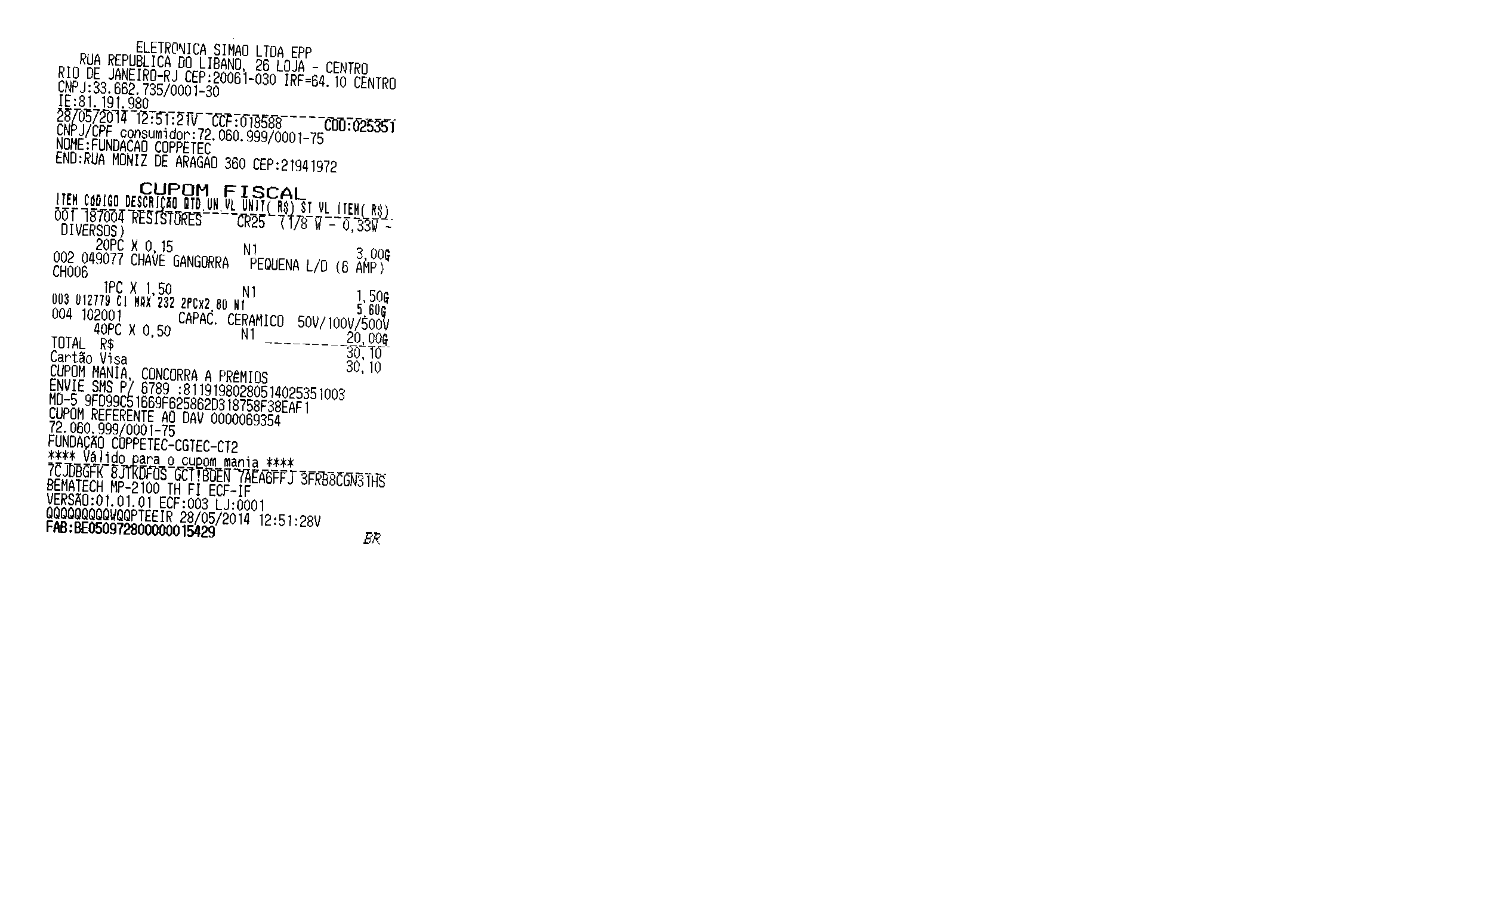
\includegraphics[width=1\columnwidth]{Componentes_Eletronicos_1/nota_eletronica1.png}
 \caption{Componentes Eletrônicos 1} 
 \end{figure}
